% GNUPLOT: LaTeX picture with Postscript
\begingroup
  \makeatletter
  \providecommand\color[2][]{%
    \GenericError{(gnuplot) \space\space\space\@spaces}{%
      Package color not loaded in conjunction with
      terminal option `colourtext'%
    }{See the gnuplot documentation for explanation.%
    }{Either use 'blacktext' in gnuplot or load the package
      color.sty in LaTeX.}%
    \renewcommand\color[2][]{}%
  }%
  \providecommand\includegraphics[2][]{%
    \GenericError{(gnuplot) \space\space\space\@spaces}{%
      Package graphicx or graphics not loaded%
    }{See the gnuplot documentation for explanation.%
    }{The gnuplot epslatex terminal needs graphicx.sty or graphics.sty.}%
    \renewcommand\includegraphics[2][]{}%
  }%
  \providecommand\rotatebox[2]{#2}%
  \@ifundefined{ifGPcolor}{%
    \newif\ifGPcolor
    \GPcolorfalse
  }{}%
  \@ifundefined{ifGPblacktext}{%
    \newif\ifGPblacktext
    \GPblacktexttrue
  }{}%
  % define a \g@addto@macro without @ in the name:
  \let\gplgaddtomacro\g@addto@macro
  % define empty templates for all commands taking text:
  \gdef\gplbacktext{}%
  \gdef\gplfronttext{}%
  \makeatother
  \ifGPblacktext
    % no textcolor at all
    \def\colorrgb#1{}%
    \def\colorgray#1{}%
  \else
    % gray or color?
    \ifGPcolor
      \def\colorrgb#1{\color[rgb]{#1}}%
      \def\colorgray#1{\color[gray]{#1}}%
      \expandafter\def\csname LTw\endcsname{\color{white}}%
      \expandafter\def\csname LTb\endcsname{\color{black}}%
      \expandafter\def\csname LTa\endcsname{\color{black}}%
      \expandafter\def\csname LT0\endcsname{\color[rgb]{1,0,0}}%
      \expandafter\def\csname LT1\endcsname{\color[rgb]{0,1,0}}%
      \expandafter\def\csname LT2\endcsname{\color[rgb]{0,0,1}}%
      \expandafter\def\csname LT3\endcsname{\color[rgb]{1,0,1}}%
      \expandafter\def\csname LT4\endcsname{\color[rgb]{0,1,1}}%
      \expandafter\def\csname LT5\endcsname{\color[rgb]{1,1,0}}%
      \expandafter\def\csname LT6\endcsname{\color[rgb]{0,0,0}}%
      \expandafter\def\csname LT7\endcsname{\color[rgb]{1,0.3,0}}%
      \expandafter\def\csname LT8\endcsname{\color[rgb]{0.5,0.5,0.5}}%
    \else
      % gray
      \def\colorrgb#1{\color{black}}%
      \def\colorgray#1{\color[gray]{#1}}%
      \expandafter\def\csname LTw\endcsname{\color{white}}%
      \expandafter\def\csname LTb\endcsname{\color{black}}%
      \expandafter\def\csname LTa\endcsname{\color{black}}%
      \expandafter\def\csname LT0\endcsname{\color{black}}%
      \expandafter\def\csname LT1\endcsname{\color{black}}%
      \expandafter\def\csname LT2\endcsname{\color{black}}%
      \expandafter\def\csname LT3\endcsname{\color{black}}%
      \expandafter\def\csname LT4\endcsname{\color{black}}%
      \expandafter\def\csname LT5\endcsname{\color{black}}%
      \expandafter\def\csname LT6\endcsname{\color{black}}%
      \expandafter\def\csname LT7\endcsname{\color{black}}%
      \expandafter\def\csname LT8\endcsname{\color{black}}%
    \fi
  \fi
  \setlength{\unitlength}{0.0500bp}%
  \begin{picture}(11520.00,8640.00)%
    \gplgaddtomacro\gplbacktext{%
      \csname LTb\endcsname%
      \put(620,640){\makebox(0,0)[r]{\strut{}-8}}%
      \csname LTb\endcsname%
      \put(620,1102){\makebox(0,0)[r]{\strut{}-7}}%
      \csname LTb\endcsname%
      \put(620,1565){\makebox(0,0)[r]{\strut{}-6}}%
      \csname LTb\endcsname%
      \put(620,2027){\makebox(0,0)[r]{\strut{}-5}}%
      \csname LTb\endcsname%
      \put(620,2490){\makebox(0,0)[r]{\strut{}-4}}%
      \csname LTb\endcsname%
      \put(620,2952){\makebox(0,0)[r]{\strut{}-3}}%
      \csname LTb\endcsname%
      \put(620,3415){\makebox(0,0)[r]{\strut{}-2}}%
      \csname LTb\endcsname%
      \put(620,3877){\makebox(0,0)[r]{\strut{}-1}}%
      \csname LTb\endcsname%
      \put(620,4340){\makebox(0,0)[r]{\strut{}0}}%
      \csname LTb\endcsname%
      \put(620,4802){\makebox(0,0)[r]{\strut{}1}}%
      \csname LTb\endcsname%
      \put(620,5264){\makebox(0,0)[r]{\strut{}2}}%
      \csname LTb\endcsname%
      \put(620,5727){\makebox(0,0)[r]{\strut{}3}}%
      \csname LTb\endcsname%
      \put(620,6189){\makebox(0,0)[r]{\strut{}4}}%
      \csname LTb\endcsname%
      \put(620,6652){\makebox(0,0)[r]{\strut{}5}}%
      \csname LTb\endcsname%
      \put(620,7114){\makebox(0,0)[r]{\strut{}6}}%
      \csname LTb\endcsname%
      \put(620,7577){\makebox(0,0)[r]{\strut{}7}}%
      \csname LTb\endcsname%
      \put(620,8039){\makebox(0,0)[r]{\strut{}8}}%
      \csname LTb\endcsname%
      \put(740,440){\makebox(0,0){\strut{}-0.5}}%
      \csname LTb\endcsname%
      \put(1608,440){\makebox(0,0){\strut{}0}}%
      \csname LTb\endcsname%
      \put(2477,440){\makebox(0,0){\strut{}0.5}}%
      \csname LTb\endcsname%
      \put(3345,440){\makebox(0,0){\strut{}1}}%
      \csname LTb\endcsname%
      \put(4213,440){\makebox(0,0){\strut{}1.5}}%
      \csname LTb\endcsname%
      \put(5081,440){\makebox(0,0){\strut{}2}}%
      \csname LTb\endcsname%
      \put(5950,440){\makebox(0,0){\strut{}2.5}}%
      \csname LTb\endcsname%
      \put(6818,440){\makebox(0,0){\strut{}3}}%
      \csname LTb\endcsname%
      \put(7686,440){\makebox(0,0){\strut{}3.5}}%
      \csname LTb\endcsname%
      \put(8554,440){\makebox(0,0){\strut{}4}}%
      \csname LTb\endcsname%
      \put(9423,440){\makebox(0,0){\strut{}4.5}}%
      \csname LTb\endcsname%
      \put(10291,440){\makebox(0,0){\strut{}5}}%
      \csname LTb\endcsname%
      \put(11159,440){\makebox(0,0){\strut{}5.5}}%
      \colorrgb{0.00,0.00,0.00}%
      \put(160,4339){\rotatebox{90}{\makebox(0,0){\strut{}Voltage ($V$)}}}%
      \colorrgb{0.00,0.00,0.00}%
      \put(5949,140){\makebox(0,0){\strut{}Voltage ($V$)}}%
      \csname LTb\endcsname%
      \put(5949,8339){\makebox(0,0){\strut{}DC Sweep of Differential Output Amplifier Input $Vin$}}%
    }%
    \gplgaddtomacro\gplfronttext{%
      \csname LTb\endcsname%
      \put(10256,4439){\makebox(0,0)[r]{\strut{}$Vout+$}}%
      \csname LTb\endcsname%
      \put(10256,4239){\makebox(0,0)[r]{\strut{}$Vout-$}}%
    }%
    \gplbacktext
    \put(0,0){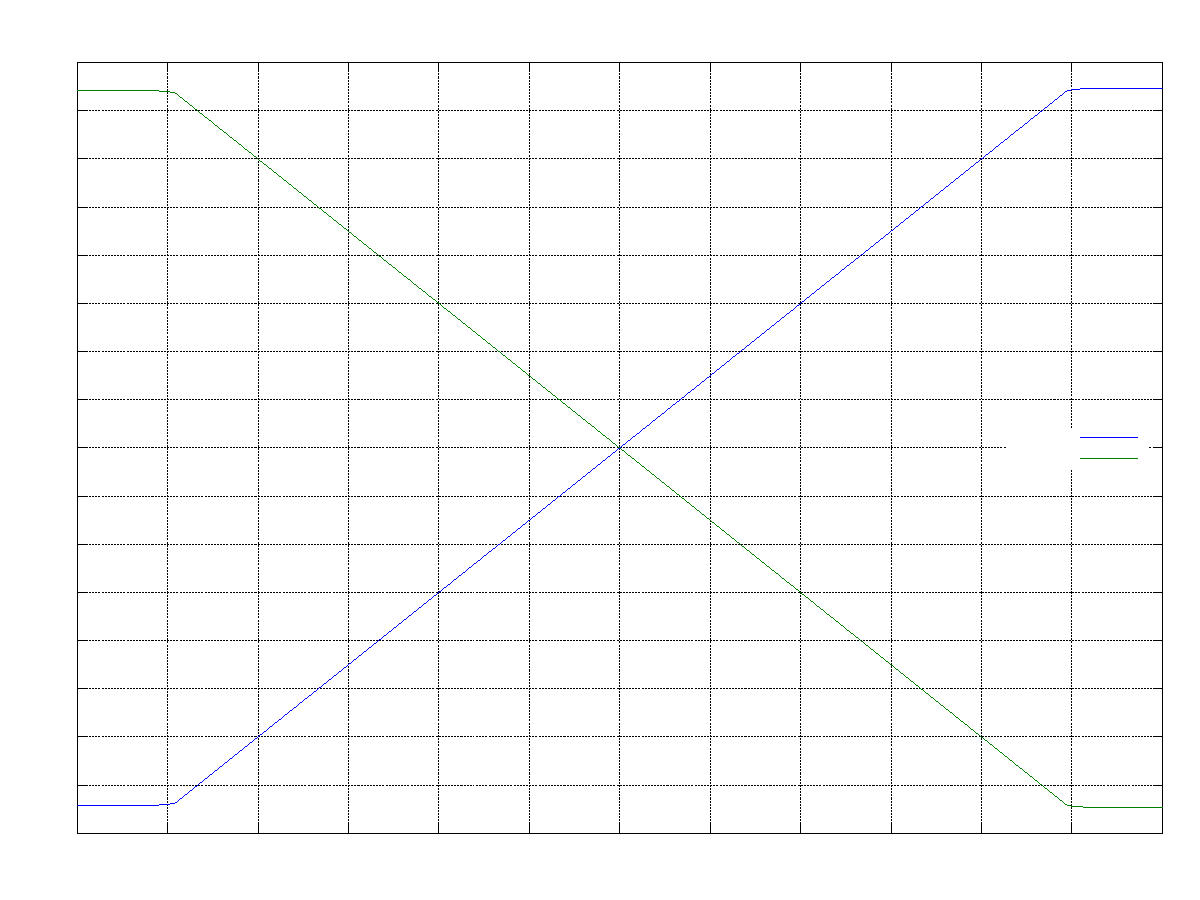
\includegraphics{DCSweep}}%
    \gplfronttext
  \end{picture}%
\endgroup
